\documentclass[11pt]{article}
\bibliographystyle{plain}
\usepackage{geometry} % see geometry.pdf on how to lay out the page. There's lots.
\usepackage{amsmath,amssymb} 
\usepackage{epsfig,epsf,subfigure}
\usepackage{listings}
\geometry{a4paper} 


%\documentclass{article}

\setlength{\parindent}{0pt}
\setlength{\parskip}{1ex plus 0.5ex minus 0.2ex}

\begin{document}
 
\LARGE
\begin{center}
TMA4280: Introduction to Supercomputing
\end{center}
\vspace{1in}

\begin{center}
{\bf Suggested solutions} \\
Problem set 1
\end{center}

\Large
\vspace{0.5in}
\begin{center}
January 2012
\end{center}

\vspace{0.5in}

\begin{center}
\copyright Einar M. R{\o}nquist \\
Department of Mathematical Sciences\\
NTNU, N-7491 Trondheim, Norway\\
All rights reserved
\end{center}

\large

\newpage

\paragraph{Exercise 1} \ \\
7 digits (single precision).

\paragraph{Exercise 2} \ \\

\begin{align*}
  4.25 &= 1 \cdot 2^2 + 0 \cdot 2^1 + 0 \cdot 2^0 + 0 \cdot 2^{-1} + 1 \cdot 2^{-2} \\
  \Rightarrow \quad (4.25)_{10} &= (100.01)_2 \\
  &= (1.0001)_2 \cdot 2^2
\end{align*}

Comparing this with (3)-(5) in the notes, we identify

\begin{align*}
  S &= 0 \\
  E-B &= 2 \quad \Rightarrow \quad E = B+2 = 127+2 = 129 \\
  \intertext{But}
  E &= (129)_{10} = (128+1)_{10} = (10000001)_2 \\
  M &= (1.0001)_2
\end{align*}
where the leading bit of $M$ is implicit in the representation.

Hence, the floating point representation of 4.25 is

\begin{figure}[!h]
  \centering
  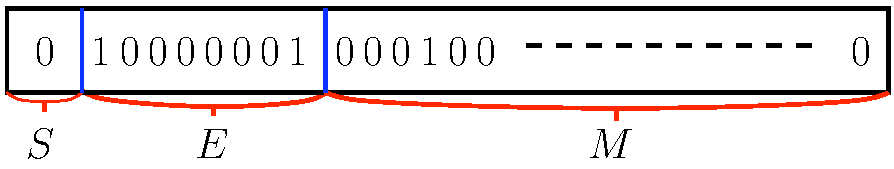
\includegraphics[width=10cm]{FloatingPointRep}
\end{figure}


\paragraph{Exercise 3} \ \\
Relative accuracy of a floating point number in double precision is $2^{-52} = 2.2 \cdot 10^{-16}$. Hence, we have $16$ digits of accuracy.

\paragraph{Exercise 4} \ \\
One alternative is to use a double loop where the inner loop only goes up to approximately $10^9$. 

Note that the data type \texttt{int} in C may only be in the 
$\pm 2^{15}$ (16 bits of information), although many newer platforms will use  
32 bits to store integer information. The data type \texttt{long} will certainly use 32 bits
for integer representation. Note that C also has the data type \texttt{long long} 
which uses 64 bits for integer representation. This alternative should certainly 
be enough as the range is $\pm 2^{63} \approx 9\cdot 10^{18}$.

\paragraph{Exercise 5} \ \\
For the first case we need $n$ additions and $n$ multiplications:

\begin{align*}
  \underline{z} &= \underline{x} + c \underline{y} \\
  &\Downarrow \\
  \mathcal{N}_{\text{ops}} &= n + n = 2n 
\end{align*}

For the matrix-vector product, the computation of each component in $\underline{y}$ requires $n$ multiplications and $n-1$ additions:
\begin{align*}
  \underline{y} &= \underline{A} \, \underline{x} \\
  &\Downarrow \\
  \mathcal{N}_{\text{ops}} &= n(n + (n-1)) = n (2n-1) \underset{\underset{n \gg 1}{\uparrow}}{\simeq} 2n^2 = \mathcal{O}(n^2). 
\end{align*}

\paragraph{Exercise 6} \ \\
Solve $\underline{A} \, \underline{x} = \underline{b}$.

Total storage requirement

\begin{equation*}
  (\underset{\underline{A}}{\underbrace{n^2}}+\underset{\underline{x}}{\underbrace{n}}+\underset{\underline{b}}{\underbrace{n}}) \cdot 8 \text{ bytes}.
\end{equation*}

Assuming that $n \gg 1$, this is approximately equal to $8 n^2$ bytes.

Constraint:

\begin{align*}
  8 n^2 &< 1 \cdot 10^9 \\
  \Rightarrow \quad n &\leq 11000.
\end{align*}

Hence, we can only solve a system with approximately $10^4$ unknowns.

\newpage
\paragraph{Code} \ \\
\lstinputlisting[language=C]{mxv.c}

\end{document}
